\documentclass[11pt,a4paper]{article}
\usepackage[utf8]{inputenc}\usepackage[T1]{fontenc}\usepackage{lmodern,textcomp}\DeclareUnicodeCharacter{2212}{\textminus}
\usepackage[margin=2.4cm]{geometry}
\usepackage{microtype,booktabs,tabularx,float,enumitem,xcolor,caption}
\usepackage{tikz,pgfplots}
\usetikzlibrary{arrows.meta}
\pgfplotsset{compat=1.18}
\usepackage[hidelinks]{hyperref}
\definecolor{accent}{HTML}{2F6FDE}\definecolor{axis}{HTML}{6B6B6B}\definecolor{quiet}{HTML}{6B6B6B}\definecolor{muted}{HTML}{B8B8B8}
\renewcommand{\arraystretch}{1.25}
\newcolumntype{X}{>{\raggedright\arraybackslash}X}
\setlist{itemsep=2pt,topsep=4pt}
\captionsetup{font=small,labelfont=bf}
\setlength{\parskip}{5pt}\setlength{\parindent}{0pt}
\title{\textbf{Learning to Play Belote with Reinforcement Learning}}
\author{Noa Curiel \& Yoni Benabou}
\date{25 October 2026}
\begin{document}
\maketitle
\begin{abstract}\noindent We trained an artificial intelligence to play two-player Belote without giving it any strategy: it learned everything by playing against itself, using the PPO method. It wins \textbf{83}\textbf{\% }\textbf{of its games} against a player who plays at random and \textbf{62}\textbf{\%} against the best strategy we wrote by hand. This result is reproduced across three independent training runs. We then added trump bidding: early results show \textbf{73.5\% of games won} against that same strategy, and better bids than those of a hand-written rule.\end{abstract}

\section*{1. Introduction}\addcontentsline{toc}{section}{1. Introduction}

\subsection*{Goal}

The project asks whether a program can learn to play Belote well \textbf{by itself}, only by playing, and rediscover or surpass the strategies of human players.

We use \textbf{reinforcement learning}. The program plays millions of games. After each one, it reinforces the choices that won it points and drops those that lost it points. Nobody explains strategy to it: it only knows the legal moves and the points won.

\subsection*{Why Belote}

\begin{itemize}

  \item \textbf{A widely played game.} It is one of the most popular card games in France, with a tournament held every year at the Technion.

  \item \textbf{A real challenge for an AI.} It is a game of \textbf{hidden information}: you cannot see your opponent's cards. In chess, everything is visible; here, every move is a bet on what the opponent holds, as in poker.

  \item \textbf{A large share of luck.} The deal weighs heavily on the outcome of a hand. Careful measurement methods are therefore needed to tell skill from luck.

  \item \textbf{A game we know.} As long-time players, we can judge whether the AI plays ``intelligently''.

\end{itemize}

\subsection*{What we built}

We wrote everything ourselves in Python, about 4,400 lines: the game engine, the learning environment, four reference opponents, the PPO method, the measurement tools, 9 automated test suites and a web app to play against the AI.

\section*{2. The starting game: Coinche}\addcontentsline{toc}{section}{2. The starting game: Coinche}

Coinche is the variant of Belote that we play. It is played by four, in two teams of two sitting opposite each other, with a 32-card deck (Ace down to 7 in all four suits). Each player receives 8 cards: every card is dealt.

\subsection*{Bidding}

Before play, players take turns announcing a \textbf{contract}: a number of points their team commits to scoring (80, 90, 100… up to 160, or ``capot'' for all the tricks), with the trump suit of their choice. Each bid must beat the previous one. Bidding ends when the other three players pass.

An opponent who thinks the contract will fail can \textbf{``coinche''}: the points at stake are doubled. The bidding team can then \textbf{``surcoinche''} to double them again.

\subsection*{Card play}

A hand is played in 8 tricks. The first player leads a card, and each player plays in turn, following three obligations:

\begin{enumerate}

  \item \textbf{Follow suit}: play a card of the suit led if you have one.

  \item \textbf{Trump}: if you have none of the suit led, play a trump (unless your partner is already winning the trick).

  \item \textbf{Overtrump}: when you play a trump, play one higher than those already on the table if you can.

\end{enumerate}

The trick is won by the highest trump or, failing that, by the highest card of the suit led. The trick winner leads the next one.

\subsection*{Card values}

The order and value of cards change in the trump suit: the Jack and the 9 rise above everything else.

\begin{table}[htbp]\centering\small\begin{tabular}{lll}\toprule

Card & Points in trumps & Points in other suits \\\midrule

Jack & \textbf{20} & 2 \\

9 & \textbf{14} & 0 \\

Ace & 11 & 11 \\

10 & 10 & 10 \\

King & 4 & 4 \\

Queen & 3 & 3 \\

8 & 0 & 0 \\

7 & 0 & 0 \\

\bottomrule\end{tabular}\end{table}

Trump order: Jack, 9, Ace, 10, King, Queen, 8, 7. Non-trump order: Ace, 10, King, Queen, Jack, 9, 8, 7.

\subsection*{Scoring}

\begin{itemize}

  \item The cards are worth 152 points in total, plus \textbf{10 points for the last trick} (``dix de der''), so 162 points per hand.

  \item The player holding \textbf{the King and Queen of trumps} scores 20 extra points (``belote, rebelote'').

  \item If the bidding team reaches its contract, it scores its points plus the contract value. Otherwise the contract \textbf{fails}: the other team scores 160 points plus the contract value, doubled if coinched.

  \item The game is played to a target set in advance, often 1,000 or 2,000 points.

\end{itemize}

Scoring details vary from table to table; these are the most common rules.

\section*{3. Our two-player adaptation}\addcontentsline{toc}{section}{3. Our two-player adaptation}

\subsection*{Why adapt}

We first programmed a complete four-player Coinche, which worked. But for learning, our professor advised us to simplify. With four players, the AI must guess three hidden hands, cooperate with a partner, share its reward with them and handle bidding. The link between a move and its outcome becomes too blurry, and learning too noisy.

So we adapted the game to two players, keeping what makes it hard: trumps, trumping and hidden information.

\subsection*{Coinche versus our version}

\begin{table}[htbp]\centering\small\begin{tabularx}{\linewidth}{lXX}\toprule

 & Coinche & Our two-player version \\\midrule

Players & 4, in two teams & 2, head to head \\

Cards in hand & 8 & 8 \\

Cards you cannot see & the hands of the other 3 players & the opponent's hand and \textbf{16 cards never dealt} \\

Choosing trumps & bidding with a contract, coinche & first drawn at random, then a simple bid on a turned-up card (section 11) \\

Bidder's commitment & reach the contract & score more points than the opponent \\

Obligations & follow suit, trump, overtrump & follow suit, trump; overtrump only when trumps are led \\

Card values & see above & identical \\

Dix de der, belote-rebelote & yes & yes \\

End of game & often 1,000 or 2,000 points & 501 points, about 10 hands \\

\bottomrule\end{tabularx}\end{table}

With 16 cards never dealt, a card you have not seen is not necessarily in the opponent's hand: deductions are trickier than with four players, where every card is in play.

We first set trumps at random so the AI could learn card play. Bidding was added only once that first goal was reached.

\section*{4. The learning environment}\addcontentsline{toc}{section}{4. The learning environment}

For an AI to learn, the game must be framed as an ``environment'': at each turn, the AI receives a description of the situation, chooses an action, then receives a reward. We built this environment with Gymnasium, the standard library in the field.

\subsection*{What the AI sees}

At each move, the AI receives a vector of \textbf{598 numbers} describing everything a human player can know:

\begin{table}[htbp]\centering\small\begin{tabularx}{\linewidth}{Xl}\toprule

Information & Size \\\midrule

The cards in its hand & 32 \\

The cards already played & 32 \\

The trump suit & 4 \\

Both players' scores & 2 \\

Who won each trick (me, the opponent, not yet played) & 8 \\

The detail of each trick: my card, the opponent's card, who led & 520 \\

\bottomrule\end{tabularx}\end{table}

The AI \textbf{never} sees the opponent's hand or the 16 undealt cards. Everything is described from its own point of view (``me'' and ``the opponent''): this is what lets the same program play either seat.

\subsection*{What it can do}

It chooses one card out of 32. Cards forbidden by the rules are \textbf{masked} before it chooses: their probability is set to zero. It can therefore never play an illegal move, and does not have to learn the rules.

\subsection*{Its reward}

It receives the points it actually wins: the points of each trick taken, the dix de der and belote-rebelote. These points are scaled between 0 and 1 to stabilise learning. The reward is therefore given hand by hand, not at the end of the 501-point game.

\section*{5. The reference opponents}\addcontentsline{toc}{section}{5. The reference opponents}

To know whether the AI is improving, it must be compared with players of known strength. We wrote four players, from weakest to strongest. Each one keeps the previous one's strategy and adds one human-player idea.

\begin{table}[htbp]\centering\small\begin{tabularx}{\linewidth}{lXXl}\toprule

Player & Strategy & Games won against Random (501 points) & Hands won against Random \\\midrule

\textbf{Random} & Plays a legal card at random. This is the floor. & 51\% & 50\% \\

\textbf{Heuristic} & Leads with its highest trump. Wins tricks with the lowest card possible. Otherwise, discards its lowest card. & 62\% & 52.9\% \\

\textbf{VoidExploit} & Spots the suits the opponent no longer holds and leads them to make it spend its trumps. & 70.7\% & 56.0\% \\

\textbf{TrumpCount} & Counts the remaining trumps and only leads trumps when it holds the majority. & \textbf{72\%} & 56.4\% \\

\bottomrule\end{tabularx}\end{table}

Games: 1,000 duplicate games of 501 points (±2 percentage points). Hands: 10,000 duplicate hands (±0.7 percentage points). See section 7. \textbf{TrumpCount}, the strongest, is the main benchmark throughout the project: it is the opponent against which we compare every version of the AI.

\section*{6. The method: PPO and self-play}\addcontentsline{toc}{section}{6. The method: PPO and self-play}

\subsection*{The neural network}

The AI is a neural network, that is, a function with many internal settings that are adjusted little by little. It takes the 598 numbers describing the situation, passes them through two layers of 128 neurons, and gives two outputs:

\begin{itemize}

  \item \textbf{the policy}: a probability of playing each legal card;

  \item \textbf{the value}: an estimate of the points it will still win in the hand.

\end{itemize}

At the start, its settings are random and it plays almost at random.

\subsection*{Self-play}

The same network plays \textbf{both players}, alternating who leads. It therefore learns against an opponent that improves at exactly the same pace. It is shown no human games and no strategy.

\subsection*{PPO}

PPO (\emph{Proximal Policy Optimization}) is one of the most widely used reinforcement learning methods. We wrote it ourselves, piece by piece, rather than using an off-the-shelf library. Training repeats a four-step loop:

\begin{figure}[H]\centering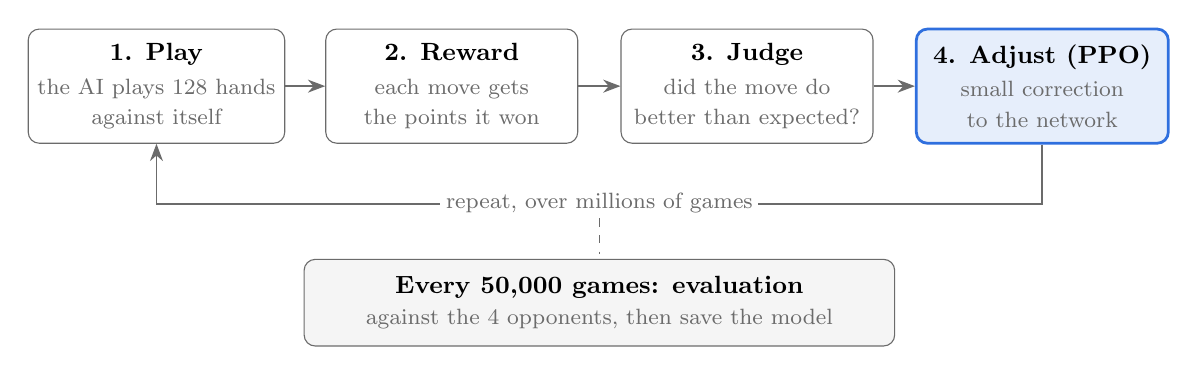
\begin{tikzpicture}[
  box/.style={draw=axis, rounded corners=4pt, minimum width=3.2cm, minimum height=1.45cm, align=center, font=\small},
  main/.style={box, draw=accent, fill=accent!12, line width=1pt},
  arr/.style={-{Stealth[length=2.2mm]}, draw=axis, line width=0.6pt}]
\node[box] (p) at (0,0) {\textbf{1. Play}\\[1pt]{\footnotesize\color{quiet}the AI plays 128 hands}\\{\footnotesize\color{quiet}against itself}};
\node[box] (r) at (3.75,0) {\textbf{2. Reward}\\[1pt]{\footnotesize\color{quiet}each move gets}\\{\footnotesize\color{quiet}the points it won}};
\node[box] (j) at (7.5,0) {\textbf{3. Judge}\\[1pt]{\footnotesize\color{quiet}did the move do}\\{\footnotesize\color{quiet}better than expected?}};
\node[main] (a) at (11.25,0) {\textbf{4. Adjust (PPO)}\\[1pt]{\footnotesize\color{quiet}small correction}\\{\footnotesize\color{quiet}to the network}};
\draw[arr] (p) -- (r); \draw[arr] (r) -- (j); \draw[arr] (j) -- (a);
\draw[arr] (a.south) -- ++(0,-0.75) -| (p.south);
\node[font=\footnotesize, text=quiet, fill=white, inner sep=2pt] at (5.625,-1.48) {repeat, over millions of games};
\draw[axis, dashed] (5.625,-1.48) ++(0,-0.2) -- ++(0,-0.45);
\node[box, minimum width=7.5cm, minimum height=1.1cm, fill=gray!8] at (5.625,-2.75) {\textbf{Every 50,000 games: evaluation}\\{\footnotesize\color{quiet}against the 4 opponents, then save the model}};
\end{tikzpicture}
\caption{the training loop}\end{figure}

\begin{enumerate}

  \item \textbf{Play.} The AI plays 128 hands against itself and records every move.

  \item \textbf{Reward.} Each move receives the points it earned.

  \item \textbf{Judge.} For each move, the points obtained are compared with what the network predicted. The difference is called the \textbf{advantage}: positive if the move did better than expected, negative otherwise.

  \item \textbf{Adjust.} Moves with a positive advantage become slightly more likely, the others slightly less. PPO \textbf{caps the size of each correction} (20\% at most) so the network does not suddenly forget what it has already learned.

\end{enumerate}

Every 50,000 games, training pauses to evaluate the AI against the four opponents and save the model.

\subsection*{Chosen settings}

\begin{table}[htbp]\centering\small\begin{tabularx}{\linewidth}{Xl}\toprule

Setting & Value \\\midrule

Hands played before each update & 128 \\

Learning passes over those hands & 4 \\

Minibatch size (moves) & 256 \\

Learning rate & 0.0003 \\

Cap on each correction & 20\% \\

Duration of a 3-million-game training run & 5 h 20 on the Technion machine \\

\bottomrule\end{tabularx}\end{table}

\section*{7. Measuring strength}\addcontentsline{toc}{section}{7. Measuring strength}

In card games, luck blurs everything. Our best hand-written strategy beats random play in only 56\% of hands. With a naive measurement over 200 games, the margin of error (±7 percentage points) was larger than the improvements we wanted to detect. So we built three tools.

\subsection*{Duplicate deals}

As in bridge tournaments, each deal is played \textbf{twice} with the hands swapped: the AI first plays hand A against hand B, then hand B against hand A. The luck of the deal cancels out, leaving only the difference in play.

\begin{table}[htbp]\centering\small\begin{tabularx}{\linewidth}{llXX}\toprule

Match-up & Hands won & Margin of error, independent deals & Margin of error, duplicate deals \\\midrule

Heuristic vs Random & 52.9\% & ±1.44 points & ±0.74 points \\

TrumpCount vs Random & 56.4\% & ±1.40 points & ±0.69 points \\

TrumpCount vs Heuristic & 55.0\% & ±1.22 points & ±0.52 points \\

VoidExploit vs Heuristic & 54.6\% & ±1.20 points & ±0.41 points \\

\bottomrule\end{tabularx}\end{table}

Margins of error on the point difference per hand, measured over 4,000 hands; percentages over 10,000 duplicate hands. The margin of error is divided by 2 to 3: 4 to 9 times fewer hands are needed for the same precision. These percentages also show how hard the game is: even between two strategies of very different strength, the better one wins only 53 to 56\% of hands.

\subsection*{The ``cheating'' player}

When we played against the AI ourselves, we lost most games. Yet it won ``only'' 63\% of hands against random play. To understand why, we programmed a player that \textbf{sees the opponent's hand} and computes the perfect move. No honest player can do better. Yet it wins only \textbf{76\% of hands} against random play: within a single hand, a bad hand cannot be saved.

\subsection*{Full 501-point games}

So we also measure strength as in a real game: first to 501 points, about 10 hands, in duplicate games. Over a whole game, luck evens out and skill shows clearly: the cheater wins 99\% of games against random play.

We therefore give two figures for each match-up: the percentage of \textbf{hands} won and the percentage of \textbf{games} won. Game measurements use 1,000 games per match-up, accurate to ±2 percentage points.

\section*{8. Debugging and tuning}\addcontentsline{toc}{section}{8. Debugging and tuning}

The first training runs ran without errors, but the AI barely improved. Two invisible bugs and a bad setting were the cause. Every fix is now checked by an automated test.

\subsection*{Two bugs that blocked learning}

\textbf{The mixed-up point of view.} The winner of each trick was recorded as ``player 0'' or ``player 1'', while everything else was described as ``me'' and ``the opponent''. Since a single network plays both seats, it could not tell who had won the previous tricks. We found it by rereading the code, and re-encoded it as ``me / opponent / not yet played''.

\textbf{Both players' points added together.} To judge a move, the advantage calculation chained the moves of both players as if they belonged to one. In a game where one player's gain is the other's loss, the signal ``this move won me points'' cancelled out. We found it while looking for why the AI was not learning. The calculation is now done separately for each player.

\subsection*{Tuning: one hypothesis at a time}

Once the bugs were fixed, the AI was still below TrumpCount. We formed four hypotheses and tested each over 200,000 games, changing only one thing at a time.

\begin{table}[htbp]\centering\small\begin{tabularx}{\linewidth}{X>{\centering\arraybackslash}p{1.75cm}>{\centering\arraybackslash}p{1.75cm}>{\centering\arraybackslash}p{1.75cm}>{\centering\arraybackslash}p{1.75cm}>{\centering\arraybackslash}p{1.75cm}}\toprule

Configuration & Hands won vs TrumpCount & Difference vs TrumpCount & vs Random & vs Heuristic & vs VoidExploit \\\midrule

Start: win bonus, fast learning & 47.9\% & −4.6 & +4.0 & −0.8 & −3.8 \\

No win bonus & 50.4\% & −0.4 & +9.8 & +0.7 & −2.0 \\

No bonus + more exploration & 51.7\% & −0.6 & +9.3 & +1.5 & −1.5 \\

No bonus + training against the heuristics & 51.0\% & −0.1 & +5.0 & +8.3 & +5.7 \\

\textbf{No bonus + slower learning} & \textbf{52.9\%} & \textbf{+1.0} & \textbf{+9.9} & \textbf{+2.6} & \textbf{+0.8} \\

\bottomrule\end{tabularx}\end{table}

Percentage of hands won against TrumpCount, then mean point difference per hand against each opponent, in duplicate deals, after 200,000 training games.

\begin{itemize}

  \item \textbf{Removing the win bonus is the decisive change.} We added ±1 to the reward depending on whether the hand was won or lost. But winning a hand depends mostly on the deal: this bonus drowned the real signal in noise.

  \item \textbf{Slower learning adds to it well.} Corrections that were too abrupt made the network oscillate. It is the only configuration that is positive against all four opponents.

  \item \textbf{More exploration brings nothing} once the bonus is removed.

  \item \textbf{Training against the heuristics specialises the AI}: it crushes them but plays worse overall. Self-play remains the best choice.

\end{itemize}

The ``no bonus + slower learning'' configuration became our default setting for all later training runs.

\section*{9. Results without bidding}\addcontentsline{toc}{section}{9. Results without bidding}

In real 501-point games, \textbf{the AI wins 83\% of its games against random play and 62\% against TrumpCount}, our best hand-written strategy. It beats all four reference opponents.

\subsection*{The main result: 501-point games}

A 501-point game lasts about 10 hands: the luck of the deal evens out, and playing strength shows clearly (section 7).

\begin{figure}[H]\centering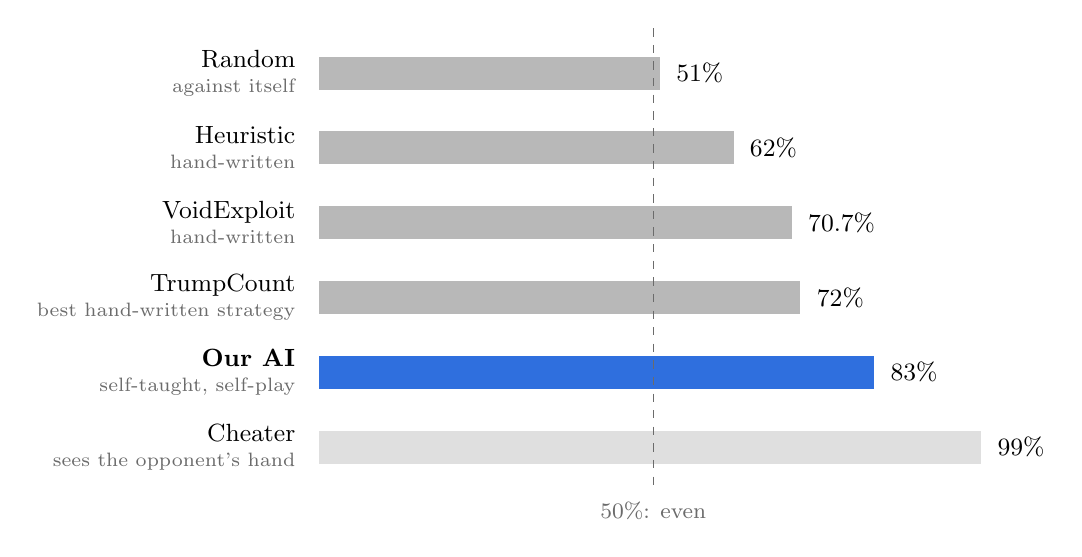
\begin{tikzpicture}[x=0.085cm, y=-0.95cm]
\foreach \i/\v/\n/\d/\c in {0/51/Random/against itself/muted, 1/62/Heuristic/hand-written/muted, 2/70.7/VoidExploit/hand-written/muted, 3/72/TrumpCount/best hand-written strategy/muted, 4/83/\textbf{Our AI}/{self-taught, self-play}/accent, 5/99/Cheater/sees the opponent's hand/muted!45}{
  \fill[\c] (0,\i-0.22) rectangle (\v,\i+0.22);
  \node[anchor=west, font=\small] at (\v+1,\i) {\v\%};
  \node[anchor=east, font=\small, align=right] at (-2,\i) {\n\\[-2pt]{\scriptsize\color{quiet}\d}};
}
\draw[dashed, axis] (50,-0.6) -- (50,5.6) node[below, font=\footnotesize, text=quiet] {50\%: even};
\end{tikzpicture}
\caption{1,000 duplicate games per player (400 for the cheater), ±2 percentage points}\end{figure}

Against random play, the AI does better than all our hand-written strategies: 83\% versus 72\% for TrumpCount. It sits between those strategies and the theoretical ceiling of the cheater, who sees the opponent's hand.

\begin{table}[htbp]\centering\small\begin{tabular}{lll}\toprule

The AI against & \textbf{Games won (501 points)} & Hands won \\\midrule

Random & \textbf{83\%} & 63\% \\

Heuristic & \textbf{72\%} & 59\% \\

VoidExploit & \textbf{64\%} & 56\% \\

TrumpCount & \textbf{62\%} & 56\% \\

\bottomrule\end{tabular}\end{table}

1,000 duplicate games per opponent, accurate to ±2 percentage points. It is the same AI, trained hand by hand: only the measurement changes between the two columns. In a single hand, the deal often decides; over a game, the better player wins much more often.

\subsection*{The learning curve}

\begin{figure}[H]\centering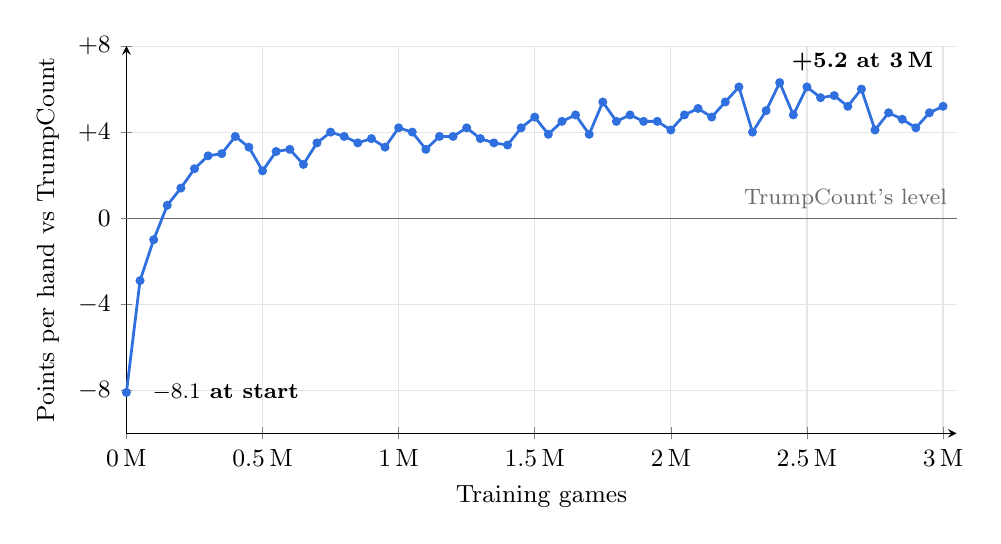
\begin{tikzpicture}
\begin{axis}[width=\linewidth, height=6.5cm, xmin=0, xmax=3.05, ymin=-10, ymax=8,
  xtick={0,0.5,...,3}, xticklabel={\pgfmathprintnumber{\tick}\,M}, ytick={-8,-4,0,4,8},
  yticklabel={\pgfmathparse{\tick>0}\ifnum\pgfmathresult=1 +\fi\pgfmathprintnumber[fixed,precision=0]{\tick}},
  xlabel={Training games}, ylabel={Points per hand vs TrumpCount},
  grid=major, grid style={draw=gray!20}, axis lines=left, tick label style={font=\small}, label style={font=\small}, clip=false]
\draw[axis] (axis cs:0,0) -- (axis cs:3.05,0) node[pos=1, above left, font=\footnotesize, text=quiet] {TrumpCount's level};
\addplot[accent, line width=1pt, mark=*, mark size=1.1pt] coordinates {(0.0000,-8.1) (0.0500,-2.9) (0.1001,-1.0) (0.1500,0.6) (0.2001,1.4) (0.2501,2.3) (0.3000,2.9) (0.3501,3.0) (0.4000,3.8) (0.4500,3.3) (0.5001,2.2) (0.5500,3.1) (0.6001,3.2) (0.6501,2.5) (0.7000,3.5) (0.7501,4.0) (0.8000,3.8) (0.8500,3.5) (0.9001,3.7) (0.9500,3.3) (1.0001,4.2) (1.0501,4.0) (1.1000,3.2) (1.1501,3.8) (1.2000,3.8) (1.2500,4.2) (1.3001,3.7) (1.3500,3.5) (1.4001,3.4) (1.4501,4.2) (1.5000,4.7) (1.5501,3.9) (1.6000,4.5) (1.6500,4.8) (1.7001,3.9) (1.7500,5.4) (1.8001,4.5) (1.8501,4.8) (1.9000,4.5) (1.9501,4.5) (2.0000,4.1) (2.0500,4.8) (2.1001,5.1) (2.1500,4.7) (2.2001,5.4) (2.2501,6.1) (2.3000,4.0) (2.3501,5.0) (2.4000,6.3) (2.4500,4.8) (2.5001,6.1) (2.5500,5.6) (2.6001,5.7) (2.6501,5.2) (2.7000,6.0) (2.7501,4.1) (2.8000,4.9) (2.8500,4.6) (2.9001,4.2) (2.9500,4.9) (3.0001,5.2)};
\node[anchor=west, font={\footnotesize\bfseries}] at (axis cs:0.06,-8.1) {$-8.1$ at start};
\node[anchor=south east, font={\footnotesize\bfseries}] at (axis cs:3.0,6.4) {+5.2 at 3\,M};
\end{axis}
\end{tikzpicture}
\caption{3-million-game training run · 1,000 duplicate hands per point}\end{figure}

The AI starts at −8 points per hand against TrumpCount, overtakes it after about 150,000 games (half an hour of training), then keeps improving more slowly.

\subsection*{The plateau}

To check that the AI is really improving, and not just against our strategies, we made it play against its own versions saved during training.

\begin{figure}[H]\centering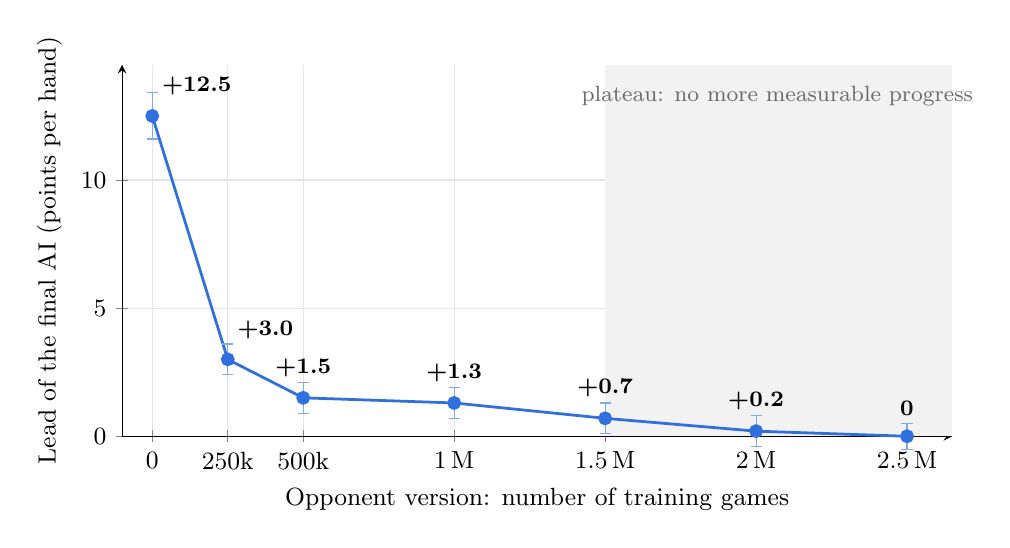
\begin{tikzpicture}
\begin{axis}[width=\linewidth, height=6.3cm, xmin=-0.1, xmax=2.65, ymin=0, ymax=14.5,
  xtick={0,0.25,0.5,1,1.5,2,2.5}, xticklabels={0,250k,500k,1\,M,1.5\,M,2\,M,2.5\,M},
  xlabel={Opponent version: number of training games}, ylabel={Lead of the final AI (points per hand)},
  axis lines=left, grid=major, grid style={draw=gray!20}, tick label style={font=\small}, label style={font=\small}, clip=false]
\fill[gray!10] (axis cs:1.5,0) rectangle (axis cs:2.65,14.5);
\node[font=\footnotesize, text=quiet] at (axis cs:2.07,13.3) {plateau: no more measurable progress};
\addplot[accent, line width=1pt, mark=*, mark size=2pt, error bars/.cd, y dir=both, y explicit, error bar style={accent!60}]
 coordinates {(0,12.5) +- (0,0.9) (0.25,3.0) +- (0,0.6) (0.5,1.5) +- (0,0.6) (1,1.3) +- (0,0.6) (1.5,0.7) +- (0,0.6) (2,0.2) +- (0,0.6) (2.5,0.0) +- (0,0.5)};
\node[font={\footnotesize\bfseries}, anchor=south west, yshift=4pt] at (axis cs:0,12.5) {+12.5};
\node[font={\footnotesize\bfseries}, anchor=south west, yshift=4pt] at (axis cs:0.25,3.0) {+3.0};
\node[font={\footnotesize\bfseries}, anchor=south, yshift=4pt] at (axis cs:0.5,1.5) {+1.5};
\node[font={\footnotesize\bfseries}, anchor=south, yshift=4pt] at (axis cs:1,1.3) {+1.3};
\node[font={\footnotesize\bfseries}, anchor=south, yshift=4pt] at (axis cs:1.5,0.7) {+0.7};
\node[font={\footnotesize\bfseries}, anchor=south, yshift=4pt] at (axis cs:2,0.2) {+0.2};
\node[font={\footnotesize\bfseries}, anchor=south, yshift=4pt] at (axis cs:2.5,0.0) {0};
\end{axis}
\end{tikzpicture}
\caption{1,000 duplicate deals per version}\end{figure}

The final AI clearly beats its early versions, but no longer beats those from after 2 million games. Learning therefore plateaus around 1.5 to 2 million games: to go further, the method must change, not just the training length.

\section*{10. What the AI learned}\addcontentsline{toc}{section}{10. What the AI learned}

By replaying deals move by move, we saw that the AI rediscovered on its own several reflexes of a good player:

\begin{itemize}

  \item \textbf{waiting} for the opponent's big trumps to fall before playing its own;

  \item \textbf{trumping} when it pays off;

  \item \textbf{keeping its master cards} to cash them at the end of the hand.

\end{itemize}

\subsection*{An example}

On one deal, trumps are diamonds. The player has strong trumps (Queen, 10, Ace and 8 of diamonds), but not the Jack or the 9, which the opponent holds.

\begin{table}[htbp]\centering\small\begin{tabularx}{\linewidth}{lXl}\toprule

Player & What it does & Points scored \\\midrule

TrumpCount & Leads the Ace of trumps, which is taken by the opponent's Jack (−31 points). & 7 \\

\textbf{Our AI} & Plays the 8 under the Jack, draws out the opponent's 9 with its Queen, then cashes its 10 and Ace, now masters. & \textbf{58} \\

\bottomrule\end{tabularx}\end{table}

\subsection*{A calculated bet, not a mistake}

In 6.6\% of its leads, the AI plays a 10 while the Ace of that suit has not yet fallen. On one lost deal, we first saw it as an oversight. Measuring over 3,000 games, we found that the opponent holds that Ace in only \textbf{15\% of cases}: with 16 cards never dealt, the Ace is most often in nobody's hand. So it is a bet that pays off 85\% of the time.

Lesson: never draw conclusions from a single deal, and measure a behaviour over thousands of games before calling it a mistake.

\subsection*{A test with no effect: the table of possible cards}

To help the AI reason about the opponent's hand, we gave it a table of the cards the opponent may still hold, deduced from the rules (if it does not follow suit, it no longer has that suit, etc.). Over two new training runs, the result is the same: +5.1 points per hand against TrumpCount, versus +4.8 without the table, a gap smaller than the measurement margin.

The explanation: all this information could already be deduced from what the AI saw, and the network had learned those deductions by itself. This negative result is useful: it shows that the AI's limit lies elsewhere.

\section*{11. Trump bidding}\addcontentsline{toc}{section}{11. Trump bidding}

\subsection*{The added rules}

Instead of drawing trumps at random, both players choose them through a bid that is simpler than Coinche bidding, modelled on classic Belote:

\begin{enumerate}

  \item One card is turned up from the 16 undealt cards and proposes its suit.

  \item \textbf{First round}: each player takes that suit or passes.

  \item \textbf{Second round}: each player names one of the other three suits or passes. If both pass again, the cards are redealt.

  \item Whoever spoke first leads the first trick.

  \item If the taker scores fewer points than the opponent, they are \textbf{``dedans''} (set): the opponent scores all the trick points.

\end{enumerate}

The AI now chooses among 38 actions: the 32 cards, take, pass, and name one of the four suits. It learns to bid and to play at the same time. It starts from our best AI without bidding, so it does not relearn card play from scratch.

\subsection*{Results}

\textbf{Provisional} results, after 350,000 training games out of the planned 2 million, in 501-point games with bidding on both sides:

\begin{table}[htbp]\centering\small\begin{tabular}{ll}\toprule

The AI against & Games won \\\midrule

Random & 98\% \\

Heuristic & 82\% \\

VoidExploit & 77\% \\

TrumpCount & \textbf{73.5\%} \\

\bottomrule\end{tabular}\end{table}

\textbf{Better bids than a hand-written rule.} We built a baseline: our previous AI for card play, plus a bidding rule we wrote (take if the suit is strong enough in the hand).

\begin{table}[htbp]\centering\small\begin{tabularx}{\linewidth}{Xl}\toprule

Player & Games won against TrumpCount \\\midrule

Previous AI + hand-written bidding & 68.8\% \\

\textbf{AI that learned to bid} & \textbf{73.5\%} \\

\bottomrule\end{tabularx}\end{table}

Head to head, the AI that learned to bid wins \textbf{54.9\% (±3.5)} of games against this baseline.

\textbf{It takes more often, and is wrong less often.} It takes trumps in 67\% of hands, twice as often as TrumpCount (33\%). Yet it is set less often when it takes: 13\% of cases versus 19\%.

These figures cannot be compared directly with the 62\% without bidding: with the ``dedans'' rule, every bad bid is very costly, which widens the gaps between players. Two 2-million-game training runs are under way to get the final figures.

\section*{12. Tools and app}\addcontentsline{toc}{section}{12. Tools and app}

\subsection*{The web app}

An app lets you play against the AI in a browser, with real cards on screen. You click a card to play it, and only legal cards are clickable. A button reveals the AI's hand, and its confidence is shown at each move. The game is played to 501 points, with the score and a log of the tricks. The AI only sees what a human player would see.

\subsection*{Tests and reliability}

\begin{itemize}

  \item \textbf{9 automated test suites} check the game, each piece of PPO, trump bidding and the reliability of training runs. Every fixed bug has its own test, so it does not come back.

  \item \textbf{Resume after interruption}: an interrupted training run picks up exactly where it left off.

  \item \textbf{Safety stop}: if an invalid value appears, training stops and saves the faulty case for analysis. This tool came from a rare crash in the bidding training runs, which we reproduced and then fixed.

  \item \textbf{Overnight watchdog}: a program automatically restarts training runs that have stopped.

\end{itemize}

\end{document}
